\section{Sobolev Spaces}
\subsection{Holder Spaces}\label{sec4.1}
Before turning to Sobolev spaces, we first discuss the simpler \textbf{Holder spaces}.\par
Assume $U\subset\mathbb{R}^n$ is open and $0<\gamma\le 1$. We have previously considered the class of Lipschitz continuous functions $u:U\to\mathbb{R}$, which by definition satisfy the estimate 
$$|u(x)-u(y)|\le C|x-y|,\hspace{0.5cm}(x,y\in U)$$
where $C$ is some constant. Now it trivially follows that a Lipschitz function is continuous and has a uniform modulus of continuity. It turns out to be useful to also consider the class of functions that satisfy 
$$|u(x)-u(y)|\le C|x-y|^\gamma,\hspace{0.5cm}(x,y\in U)$$
where $C$ is a constant and $0<\gamma\le 1$. Such a function is called a \textbf{Holder function}.
\begin{definition}
If $u:U\to\mathbb{R}$ is bounded and continuous, we write 
$$\|u\|_{C(\overline{U})}=\sup_{x\in U}|u(x)|.$$
The \textbf{$\gamma$-th Holder seminorm} of $u$ is defined to be 
$$
\left[ u \right] _{C^{0,\gamma}(\overline{U})}=\mathop {\mathrm{sup}} \limits_{x,y\in U,x\ne y}\left\{ \frac{\left| u\left( x \right) -u\left( y \right) \right|}{\left| x-y \right|^{\gamma}} \right\} ,
$$
and the \textbf{$\gamma$-th Holder norm} is 
$$
\left\| u \right\| _{C^{0,\gamma}(\overline{U})}=\left\| u \right\| _{C^{0,\gamma}(\overline{U})}+\left[ u \right] _{C^{0,\gamma}(\overline{U})}.
$$
The \textbf{Holder space} $C^{k,\gamma}(\overline{U})$ consists of all functions $u\in C^k(\overline{U})$ for which the norm 
$$
\left\| u \right\| _{C^{0,\gamma}(\overline{U})}=\sum_{\left| \alpha \right|\le k}{\left\| D^{\alpha}u \right\| _{C(\overline{U})}}+\sum_{\left| \alpha \right|=k}{\left[ D^{\alpha}u \right] _{C^{0,\gamma}(\overline{U})}}
$$
is finite.
\end{definition}
So that $C^{k,\gamma}$ consists of those functions $u$ that are $k$-times continuously differentiable and whose $k$-th partial derivatives are bounded and Holder continuous with exponent $\gamma$. Such functions are well-behaved, and furthermore the space $C^{k,\gamma}(\overline{U})$ itself possesses a good mathematical structure.
\begin{theorem}
The space of functions $C^{k,\gamma}(\overline{U})$ is a Banach space.
\end{theorem}
\begin{proof}
It suffices to show that $\|\cdot\|_{C^{k,\gamma}(\overline{U})}$ is indeed a norm, and the space $C^{k,\gamma}(\overline{U})$ is complete.\par
We first show that $\|\cdot\|_{C^{k,\gamma}(\overline{U})}$ is a norm. Suppose $u$ and $v$ are two elements of $C^{k,\gamma}(\overline{U})$. Firstly we have 
$$
\begin{aligned}
\left\| u+v \right\| _{C^{0,\gamma}(\overline{U})}&=\sum_{\left| \alpha \right|\le k}{\left\| D^{\alpha}\left( u+v \right) \right\| _{C(\overline{U})}}+\sum_{\left| \alpha \right|=k}{\left[ D^{\alpha}\left( u+v \right) \right] _{C^{0,\gamma}(\overline{U})}}
\\
&\le \sum_{\left| \alpha \right|\le k}{\left\| D^{\alpha}u \right\| _{C(\overline{U})}+\left\| D^{\alpha}v \right\| _{C(\overline{U})}}+\sum_{\left| \alpha \right|=k}{\mathop {\mathrm{sup}} \limits_{x,y\in U,x\ne y}\left\{ \frac{\left| u\left( x \right) -u\left( y \right) \right|+\left| v\left( x \right) -v\left( y \right) \right|}{\left| x-y \right|^{\gamma}} \right\}}
\\
&\le \sum_{\left| \alpha \right|\le k}{\left\| D^{\alpha}u \right\| _{C(\overline{U})}+\left\| D^{\alpha}v \right\| _{C(\overline{U})}}+\sum_{\left| \alpha \right|=k}{\mathop {\mathrm{sup}} \limits_{x,y\in U,x\ne y}\left\{ \frac{\left| u\left( x \right) -u\left( y \right) \right|}{\left| x-y \right|^{\gamma}} \right\} +\mathop {\mathrm{sup}} \limits_{x,y\in U,x\ne y}\left\{ \frac{\left| v\left( x \right) -v\left( y \right) \right|}{\left| x-y \right|^{\gamma}} \right\}}
\\
&=\sum_{\left| \alpha \right|\le k}{\left\| D^{\alpha}u \right\| _{C(\overline{U})}}+\sum_{\left| \alpha \right|=k}{\left[ D^{\alpha}u \right] _{C^{0,\gamma}(\overline{U})}}+\sum_{\left| \alpha \right|\le k}{\left\| D^{\alpha}v \right\| _{C(\overline{U})}}+\sum_{\left| \alpha \right|=k}{\left[ D^{\alpha}v \right] _{C^{0,\gamma}(\overline{U})}}
\\
&=\left\| u \right\| _{C^{0,\gamma}(\overline{U})}+\left\| v \right\| _{C^{0,\gamma}(\overline{U})}.
\end{aligned}
$$
Now suppose $\lambda\in\mathbb{R}$, therefore 
$$
\begin{aligned}
\left\| \lambda u \right\| _{C^{0,\gamma}(\overline{U})}&=\sum_{\left| \alpha \right|\le k}{\left\| D^{\alpha}\lambda u \right\| _{C(\overline{U})}}+\sum_{\left| \alpha \right|=k}{\left[ D^{\alpha}\lambda u \right] _{C^{0,\gamma}(\overline{U})}}
\\
&=\left| \lambda \right|\cdot \sum_{\left| \alpha \right|\le k}{\left\| D^{\alpha}u \right\| _{C(\overline{U})}}+\left| \lambda \right|\cdot \sum_{\left| \alpha \right|=k}{\left[ D^{\alpha}u \right] _{C^{0,\gamma}(\overline{U})}}
\\
&=\left| \lambda \right|\cdot \left( \sum_{\left| \alpha \right|\le k}{\left\| D^{\alpha}u \right\| _{C(\overline{U})}}+\sum_{\left| \alpha \right|=k}{\left[ D^{\alpha}u \right] _{C^{0,\gamma}(\overline{U})}} \right) 
\\
&=\left| \lambda \right|\cdot \left\| u \right\| _{C^{0,\gamma}(\overline{U})}.
\end{aligned}
$$
If $\|u\|_{C^{k,\gamma}(\overline{U})}=0$, then 
$$
\sum_{\left| \alpha \right|\le k}{\left\| D^{\alpha}u \right\| _{C(\overline{U})}}+\sum_{\left| \alpha \right|=k}{\left[ D^{\alpha}u \right] _{C^{0,\gamma}(\overline{U})}}=0.
$$
Hence $\|D^{\alpha}u\|_{C(\overline{U})}=0$ for all $0\le\alpha\le k$ and $[D^\alpha u]_{C^{0,\gamma}(\overline{U})}=0$ for all $|\alpha|=k$. Therefore $u=0$. The converse condition is trivial.\par
Now it suffices to show that $C^{k,\gamma}(\overline{U})$ is complete. To do this, we observe that the space $C^k(\overline{U})$ is complete. Therefore suppose $\{u_n\}_{n=1}^\infty$ is a Cauchy sequence in $C^{k,\gamma}(\overline{U})$, we have 
$$
\sum_{\left| \alpha \right|\le k}{\left\| D^{\alpha}\left( u_n-u_m \right) \right\| _{C(\overline{U})}}+\sum_{\left| \alpha \right|=k}{\left[ D^{\alpha}\left( u_n-u_m \right) \right] _{C^{0,\gamma}(\overline{U})}}<\varepsilon .
$$
Hence we have $D^\alpha u_n\to D^\alpha u$ for some $u\in C^k(\overline{U})$. Now it suffices to show that $u_n\to u$ with respect to the norm of Holder space. Note that 
$$
\sum_{\left| \alpha \right|=k}{\left[ D^{\alpha}\left( u_n-u_m \right) \right] _{C^{0,\gamma}(\overline{U})}}=\sum_{\left| \alpha \right|=k}{\mathop {\mathrm{sup}} \limits_{x,y\in U,x\ne y}\left\{ \frac{D^{\alpha}\left( u_n-u \right) \left( x \right) -D^{\alpha}\left( u_n-u \right) \left( y \right)}{\left| x-y \right|^{\gamma}} \right\}}\rightarrow 0
$$
as $n\to\infty$, we have $u_n\to u$.
\end{proof}
\subsection{Sobolev Spaces}
The Holder space introduced in section \ref{sec5.1} is unfortunately not often suitable settings for elementary PDE theory, since we usually can't make good enough analytic estimates to demonstrate that the solutions we construct actually belong to such spaces. What are needed rather are some other kinds of spaces, containing less smooth functions. In practice we must strike a balance, by designing spaces comprising functions which have some, but not too great, smoothness properties.\par
We start off by substantially weakening the notion of partial derivatives. Lets denote $C_c^\infty(U)$ the space of infinitely differentiable functions $\phi:U\to\mathbb{R}$ with compact support in $U$. We will sometimes call a function $\phi$ belonging to $C_c^\infty(U)$ a \textbf{test function}.\par
Assume we are given a function $u\in C^k(U)$ and $\phi$ a test function. We may integrate by parts to obtain 
\begin{equation}\label{4.1}
\int_U{u\cdot D^{\alpha}\phi \mathrm{d}x}=\left( -1 \right) ^{\left| \alpha \right|}\int_U{D^{\alpha}u\cdot \phi \mathrm{d}x},
\end{equation}
where $\alpha$ is a multiindex of order $k$. Our question is whether some variant of it might still be true even if $u$ is not $k$ times differentiable. Now if $u$ is not in $C^k(U)$, clearly $D^\alpha u$ makes no sense. However, we may resolve the difficulty by asking there exists a locally summable function $v$ for which the formula \eqref{4.1} is still valid. This motivates us to introduce the following definition.
\begin{definition}
Suppose $u,v\in L_{\mathrm{loc}}^1(U)$ and $\alpha$ is a multiindex. We say that $v\in L_{\mathrm{loc}}^1(U)$ is the $\alpha$-th weak partial derivative of $u$, written $D^\alpha u=v$, provided 
\begin{equation}\label{4.2}
\int_U{u\cdot D^{\alpha}\phi \mathrm{d}x}=\left( -1 \right) ^{\left| \alpha \right|}\int_U{v\cdot \phi \mathrm{d}x}.
\end{equation}
for all test functions $\phi\in C_c^\infty(U)$.
\end{definition}
In other words, if we are given $u$ and if there happens to exist a function $v$ which verifies \eqref{4.2} for all $\phi\in C_c^\infty(U)$, we say that $D^\alpha u=v$ in a weak sense.
\begin{lemma}\em
A weak $\alpha$-th partial derivative of $u$, if it exists, is defined up to a set of measure zero.
\end{lemma}
\begin{proof}
Assume that $v$ and $\widetilde{v}$ both are the weak derivative of $u$. Then 
$$
\left( -1 \right) ^{\alpha}\int_U{\left( v-\widetilde{v} \right) \cdot \phi \mathrm{d}x}=\left( -1 \right) ^{\left| \alpha \right|}\int_U{v\cdot \phi \mathrm{d}x}-\left( -1 \right) ^{\left| \alpha \right|}\int_U{\widetilde{v}\cdot \phi \mathrm{d}x}=0,
$$
hence $v=\widetilde{v}$ a.e.
\end{proof}
We now give some examples of weak derivatives.
\begin{example}\em
Let $n=1$, $U=(0,2)$, and 
$$
u\left( x \right) =\chi _{\left( 0,1 \right]}\left( x \right) \cdot x+\chi _{\left[ 1,2 \right)}\left( x \right) .
$$
We show that the weak derivative of $u$ is $\chi_{(0,1]}$. To see this, choose any $\phi\in C_c^\infty(U)$, we have 
$$
\int_U{u\cdot \phi ^{\prime}\mathrm{d}x}=\int_0^2{u\cdot \phi ^{\prime}\mathrm{d}x}=\int_0^1{u\cdot \phi ^{\prime}\mathrm{d}x}+\int_1^2{u\cdot \phi ^{\prime}\mathrm{d}x}=-\int_0^1{u^{\prime}\cdot \phi \mathrm{d}x}+\phi \left( 1 \right) -\phi \left( 1 \right) =-\int_0^2{\chi _{\left( 0,1 \right]}\cdot \phi \mathrm{d}x}.
$$
However, if we consider 
$$
u\left( x \right) =\chi _{\left( 0,1 \right]}\left( x \right) \cdot x+2\chi _{\left( 1,2 \right)}\left( x \right) ,
$$
we claim that the weak derivative of $u$ does not exist. We prove by contradiction. Suppose $v$ is a weak derivative of $u$, then for all $\phi\in C_c^\infty(U)$ we have 
$$
-\int_0^2{v\cdot \phi \mathrm{d}x}=\int_0^2{v\cdot \phi ^{\prime}\mathrm{d}x}=\int_0^1{x\cdot \phi ^{\prime}\mathrm{d}x}+2\int_1^2{\phi ^{\prime}\mathrm{d}x}=-\int_0^1{\phi \mathrm{d}x}-\phi \left( 1 \right) .
$$
Choose a sequence $\{\phi_m\}_{m=1}^\infty$ of smooth functions satisfying 
$$
0\le \phi _m\le 1,\hspace{0.5cm}\phi _m\left( 1 \right) =1,\hspace{0.5cm}\phi _m\left( x \right) \rightarrow 0\ \text{for all}\ x\ne 1.
$$
Therefore we have 
$$
1=\lim_{m\rightarrow \infty} \phi _m\left( 1 \right) =\lim_{m\rightarrow \infty} \left( \int_0^2{v\cdot \phi _m\mathrm{d}x}-\int_0^1{\phi _m\mathrm{d}x} \right) =0,
$$
a contradiction!
\end{example}
We shall now define certain function spaces, whose members have weak derivatives of various orders lying in various $L^p$ spaces.
\begin{definition}
The \textbf{Sobolev space} $W^{k,p}(U)$ consists of all locally summable functions $u:U\to\mathbb{R}$ such that for each multiindex $\alpha$ with $|\alpha|\le k$, $D^\alpha u$ exists in the weak sense and belongs to $L^p(U)$.
\end{definition}
\begin{note}\em
(i) If $p=2$, we shall write $H^k(U)=W^{k,2}(U)$ for $k=0,1,\cdots$. The letter $H$ is used since, as we will see, $H^k(U)$ is a Hilbert space. Note that $H^0(U)=L^2(U)$.\par
(ii) We henceforth identify functions in $W^{k,p}(U)$ which agree a.e.
\end{note}
Now if $u\in W^{k,p}(U)$, we define its norm to be 
$$
\left\| u \right\| _{W^{k,p}\left( U \right)}=\left\{ \begin{aligned}
	\left( \sum_{\left| \alpha \right|\le k}{\int_U{\left| D^{\alpha}u \right|^p\mathrm{d}x}} \right) ^{\frac{1}{p}}&\ \left( 1\le p<\infty \right)\\
	\sum_{\left| \alpha \right|\le k}{\mathop {\mathrm{ess} \mathrm{sup}} \limits_{U}\left| D^{\alpha}u \right|}&\ \left( p=\infty \right)\\
\end{aligned} \right. 
$$
We write $u_m\to u$ in $W_{\mathrm{loc}}^{k,p}(U)$, if $u_m\to u$ in $W^{k,p}(V)$ for each $V\subset\subset U$.\par
We shall now give a characterization of functions in $W^{1,p}(U)$ when $U\subset\mathbb{R}$. Suppose $U=(a,b)$ (may be infinite).
\begin{proposition}\label{Prop4.2.3}
Suppose $u\in W^{1,p}(U)$, then $u$ equals a.e. to an absolutely continuous function whose ordinary derivative belongs to $L^p(U)$.
\end{proposition}
In order to prove Proposition \ref{Prop4.2.3}, we shall first give two lemmas. Note that we shall only work on $L^1$ spaces and the $L^p$ space condition follows analogously. Our proof is due to Brezis \cite{brezis2011functional}.
\begin{lemma}\em
If $f\in L_{\mathrm{loc}}^1(U)$ such that for all test function $\phi$, we have 
$$
\int_U{f\phi ^{\prime}\mathrm{d}x}=0,
$$
then $f=C$ a.e. for some constant $C$.
\end{lemma}
\begin{proof}
Fix a test function $\psi$ such that $\int_U\psi=1$. For all $w\in C_c(U)$, consider $h=w-\left(\int_U w\mathrm{d}x\right)\cdot\psi$. Trivially $h$ is compactly supported, therefore there exists some $\phi\in C_c^1(U)$ such that $\phi^\prime=h$. Therefore 
$$
\int_U{f\left[ w-\left( \int_U{w} \right) \cdot \psi \right] \mathrm{d}x}=\int_U{fw\mathrm{d}x}-\left( \int_U{w\mathrm{d}x} \right) \cdot \int_U{w\psi \mathrm{d}x}=\int_U{w\cdot \left[ f-\int_U{f\psi \mathrm{d}y} \right] \mathrm{d}x}=0,
$$
however $w$ is chosen arbitrarily, therefore it follows that $f=\int_U{f\psi \mathrm{d}y}$ a.e., which is a constant.
\end{proof}
\begin{lemma}\em
Suppose $g\in L_{\mathrm{loc}}^1(U)$, define 
$$
v\left( x \right) =\int_{y_0}^x{g\left( t \right) \mathrm{d}t},
$$
then $v\in C(U)$ and 
$$
\int_U{v\phi ^{\prime}}=-\int_U{g\phi}
$$
for all test function $\phi$.
\end{lemma}
\begin{proof}
We apply Fubini's theorem. Note that 
$$
\begin{aligned}
\int_U{v\left( x \right) \phi ^{\prime}\left( x \right) \mathrm{d}x}&=\int_a^b{\left[ \int_{y_0}^x{g\left( t \right) \mathrm{d}t} \right] \phi ^{\prime}\left( x \right) \mathrm{d}x}
\\
&=\int_a^{y_0}{\phi ^{\prime}\left( x \right) \mathrm{d}x\int_{y_0}^x{g\left( t \right) \mathrm{d}t}}+\int_{y_0}^b{\phi ^{\prime}\left( x \right) \mathrm{d}x\int_{y_0}^x{g\left( t \right) \mathrm{d}t}}
\\
&=-\int_a^{y_0}{\phi ^{\prime}\left( x \right) \mathrm{d}x\int_x^{y_0}{g\left( t \right) \mathrm{d}t}}+\int_{y_0}^b{\phi ^{\prime}\left( x \right) \mathrm{d}x\int_{y_0}^x{g\left( t \right) \mathrm{d}t}}
\\
&=-\int_a^{y_0}{g\left( t \right) \mathrm{d}t\int_a^t{\phi ^{\prime}\left( x \right) \mathrm{d}x}}+\int_{y_0}^b{g\left( t \right) \mathrm{d}t\int_t^b{\phi ^{\prime}\left( x \right) \mathrm{d}x}}
\\
&=-\int_a^{y_0}{g\left( t \right) \left[ \phi \left( t \right) -\phi \left( a \right) \right] \mathrm{d}t}+\int_{y_0}^b{g\left( t \right) \left[ \phi \left( b \right) -\phi \left( t \right) \right] \mathrm{d}t}
\\
&=-\int_a^b{g\left( t \right) \phi \left( t \right) \mathrm{d}t}.
\end{aligned}
$$
Therefore the proof is finished.
\end{proof}
Now we proof Proposition \ref{Prop4.2.3}.
\begin{proof}
Define 
$$
\overline{u}=\int_{y_0}^x{u^{\prime}\left( t \right) \mathrm{d}t}.
$$
Then we have 
$$
\int_U{\overline{u}\phi ^{\prime}\mathrm{d}x}=-\int_U{u^{\prime}\phi \mathrm{d}x}=\int_U{u\phi ^{\prime}\mathrm{d}x},
$$
therefore 
$$
\int_U{\left( \overline{u}-u \right) \phi ^{\prime}}=0,
$$
and hence $\overline{u}=u+C$ a.e. for some constant $C$. Hence the function $\overline{u}+C$ satisfies the conditions.
\end{proof}
\begin{note}\em
Note that however, such characterization is only valid when $n=1$. For higher dimensions, a function that is discontinuous or unbounded may also belong to a Sobolev space.
\end{note}
\begin{example}\em
Take $U=B(0,1)$, the open unit ball in $\mathbb{R}^n$, and 
$$u(x)=|x|^{-\alpha},\hspace{0.5cm}(x\in U,x\ne 0)$$
for which values of $\alpha>0$, $n$ and $p$ does $u$ belong to $W^{1,p}(U)$? To answer, note first that $u$ is smooth away the origin, with 
$$
\left| Du\left( x \right) \right|=\left( \sum_{i=1}^n{\left| u_{x_i}\left( x \right) \right|^2} \right) ^{\frac{1}{2}}=\left( \sum_{i=1}^n{\left| \frac{-\alpha x_i}{\left| x \right|^{\alpha +2}} \right|^2} \right) ^{\frac{1}{2}}=\frac{\left| \alpha \right|}{\left| x \right|^{\alpha +2}}\cdot \left| x \right|=\frac{\left| \alpha \right|}{\left| x \right|^{\alpha +1}}.
$$
Let $\varepsilon>0$ and $\phi$ a test function. Then 
$$
\int_{U\setminus B\left( 0,\varepsilon \right)}{u\phi _{x_i}\mathrm{d}x}=-\int_{U\setminus B\left( 0,\varepsilon \right)}{u_{x_i}\phi \mathrm{d}x}+\int_{\partial B\left( 0,\varepsilon \right)}{u\phi \nu ^i\mathrm{d}S}.
$$
Now if $\alpha+1<n$, we have $|Du(x)|\in L^1(U)$. In this case 
$$
\left| \int_{\partial B\left( 0,\varepsilon \right)}{u\phi \nu ^i\mathrm{d}S} \right|\le \left\| \phi \right\| _{\infty}\cdot \int_{\partial B\left( 0,\varepsilon \right)}{\varepsilon ^{-\alpha}\mathrm{d}S}=C\varepsilon ^{n-1-\alpha}\rightarrow 0
$$
and hence 
$$
\int_{U\setminus B\left( 0,\varepsilon \right)}{u\phi _{x_i}\mathrm{d}x}=-\int_{U\setminus B\left( 0,\varepsilon \right)}{u_{x_i}\phi \mathrm{d}x}
$$
for all $\phi\in C_c^\infty(U)$ provided $0\le\alpha<n-1$. Furthermore $|Du(x)|\in L^p(U)$ if and only if $(\alpha+1)p<n$. Consequently $u\in W^{1,p}(U)$ if and only if $\alpha<(n-p)/p$.
\end{example}
\begin{example}\em
Let $\{r_k\}_{k=1}^\infty$ be a countable, dense subset of $U=B(0,1)$. Write 
$$
u\left( x \right) =\sum_{k=1}^{\infty}{\frac{\left| x-r_k \right|^{-\alpha}}{2^k}},\hspace{0.5cm}\left( x\in U \right) 
$$
then $u\in W^{1,p}(U)$ for $\alpha<(n-p)/p$. However, if $0<\alpha<(n-p)/p$, we see that $u$ belongs to $W^{1,p}(U)$ and yet is unbounded on each open subset of $U$.
\end{example}
\begin{note}\em
This last example illustrates a fundamental fact of life, that although a function $u$ belonging to a Sobolev space possesses certain smoothness properties, it can still be rather badly behaved in other ways.
\end{note}
Next we verify certain properties of weak derivatives. Note very carefully that whereas these various rules are obviously true for smooth functions, functions in Sobolev space are not necessarily continuous or bounded, we must always rely solely upon the definition of weak derivatives.
\begin{theorem}
Assume $u,v\in W^{k,p}(U)$, $|\alpha|\le k$. Then \par
(i) $D^\alpha u\in W^{k-|\alpha|,p}(U)$ and $D^{\beta}(D^{\alpha}u)=D^{\alpha+\beta}u$ for all multiindices $\alpha$, $\beta$ with $|\alpha|+|\beta|\le k$.\par
(ii) For each $\lambda,\mu\in\mathbb{R}$, $\lambda u+\mu v\in W^{k,p}(U)$ and $D^{\alpha}(\lambda u+\mu v)=\lambda D^{\alpha}u+\mu D^{\beta}v$, $|\alpha|\le k$.\par
(iii) If $V$ is an open subset of $U$, then $u\in W^{k,p}(V)$.\par
(iv) If $\zeta\in C_c^\infty(U)$, then $\zeta u\in W^{k,p}(U)$ and 
$$
D^{\alpha}\left( \zeta u \right) =\sum_{\beta \le \alpha}{C_{\alpha}^{\beta}D^{\beta}\zeta D^{\alpha -\beta}u},
$$
where $C_{\alpha}^{\beta}=\alpha !/\left[ \beta !\left( \alpha -\beta \right) ! \right] $.
\end{theorem}
\begin{proof}
Fix a test function $\phi\in C_c^\infty(U)$. We shall prove by definition.
(i) Since $u$ has weak derivative up to order $k$, trivially $D^\alpha u$ has weak derivative up to order $k-|\alpha|$. Now we show that $D^\beta(D^\alpha u)=D^{\alpha+\beta}(u)$. Observe that 
$$
\int_U{D^{\alpha}u\cdot D^{\beta}\phi \mathrm{d}x}=\left( -1 \right) ^{\left| \alpha \right|}\int_U{u\cdot D^{\alpha +\beta}\phi \mathrm{d}x}=\left( -1 \right) ^{\left| \alpha \right|}\cdot \left( -1 \right) ^{\left| \alpha +\beta \right|}\int_U{D^{\alpha +\beta}u\cdot \phi \mathrm{d}x},
$$
we have $D^\beta(D^\alpha u)=D^{\alpha+\beta}(u)$.\par
(ii) Observe that 
$$
\begin{aligned}
\int_U{\left( \lambda u+\mu v \right) \cdot D^{\alpha}\phi \mathrm{d}x}&=\lambda \int_U{u\cdot D^{\alpha}\phi \mathrm{d}x}+\mu \int_U{v\cdot D^{\alpha}\phi \mathrm{d}x}
\\
&=\lambda \int_U{D^{\alpha}u\cdot \phi \mathrm{d}x}+\mu \int_U{D^{\alpha}v\cdot \phi \mathrm{d}x}
\\
&=\int_U{\left( \lambda D^{\alpha}u+\mu D^{\alpha}v \right) \cdot \phi \mathrm{d}x},
\end{aligned}
$$
therefore $\lambda u+\mu v\in W^{k,p}(U)$ and $D^{\alpha}(\lambda u+\mu v)=\lambda D^{\alpha}u+\mu D^{\beta}v$, $|\alpha|\le k$.\par
(iii) Choose $\psi\in C_c^\infty(V)$. Then clearly $\psi\in C_c^\infty(U)$. Therefore 
$$
\int_V{u\cdot D^{\alpha}\psi \mathrm{d}x}=\int_V{D^{\alpha}u\cdot \psi \mathrm{d}x}
$$
and hence $u\in W^{k,p}(V)$.\par
(iv) We prove by induction. Suppose $|\alpha|=1$, then 
$$
\int_U{\zeta uD^{\alpha}\phi \mathrm{d}x}=\int_U{uD^{\alpha}\left( \zeta \phi \right) -u\left( D^{\alpha}\zeta \right) \phi \mathrm{d}x}=\int_U{u\mathrm{d}\zeta \phi}-\int_U{u\left( D^{\alpha}\zeta \right) \phi \mathrm{d}x}=\int_U{\left( \zeta D^{\alpha}u+uD^{\alpha}\zeta \right) \phi \mathrm{d}x}.
$$
Therefore we have $D^\alpha(\zeta u)=\zeta D^\alpha u+uD^\alpha\zeta$. Now assume $l<k$ and the statement is true for all $|\alpha|\le l$. Now suppose $|\alpha|=l+1$. Then there exists some $|\beta|=l$, $|\gamma|=1$ such that $\alpha=\beta+\gamma$. Now by induction hypothesis we have 
$$
\begin{aligned}
\int_U{\zeta uD^{\alpha}\phi \mathrm{d}x}&=\int_U{\zeta uD^{\beta}\left( D^{\alpha}\phi \right) \mathrm{d}x}
\\
&=\left( -1 \right) ^{\left| \beta \right|}\int_U{\sum_{\sigma \le \beta}{C_{\beta}^{\sigma}D^{\sigma}\zeta D^{\beta -\sigma}uD^{\gamma}\phi \mathrm{d}x}}
\\
&=\left( -1 \right) ^{\left| \beta \right|+\left| \gamma \right|}\int_U{\sum_{\sigma \le \beta}{C_{\beta}^{\sigma}D^{\gamma}\left( D^{\sigma}\zeta D^{\beta -\sigma}u \right)}\cdot \phi \mathrm{d}x}
\\
&=\left( -1 \right) ^{\left| \alpha \right|}\int_U{\sum_{\sigma \le \beta}{C_{\beta}^{\sigma}\left[ D^{\rho}\zeta D^{\alpha -\rho}u+D^{\sigma}\zeta D^{\alpha -\sigma}u \right]}\cdot \phi \mathrm{d}x}
\\
&=\left( -1 \right) ^{\alpha}\int_U{\left( \sum_{\sigma \le \beta}{C_{\alpha}^{\sigma}D^{\sigma}\zeta D^{\alpha -\sigma}u} \right) \cdot \phi \mathrm{d}x},
\end{aligned}
$$
where $\rho=\sigma+\gamma$, and the last step follows from the fact that $C_{\beta}^{\sigma-\gamma}+C_{\beta}^{\sigma}=C_{\alpha}^{\sigma}$.
\end{proof}
Not only do many of the usual rules of calculus apply to weak derivatives, but the Sobolev space itself have a good mathematical structure.
\begin{theorem}
For each $k=1,2,\cdots$ and $1\le p\le\infty$, the Sobolev space $W^{k,p}(U)$ is a Banach space.
\end{theorem}
\begin{proof}
We shall first check that $\|\cdot\|_{W^{k,p}(U)}$ is a norm. Suppose first $1\le p<\infty$. Then trivially $\|u\|_{W^{k,p}(U)}\ge 0$. Also observed that 
$$
\begin{aligned}
\left\| u+v \right\| _{W^{k,p}\left( U \right)}&=\left( \sum_{\left| \alpha \right|\le k}{\int_U{\left| D^{\alpha}\left( u+v \right) \right|^p\mathrm{d}x}} \right) ^{\frac{1}{p}}=\left( \sum_{\left| \alpha \right|\le k}{\left\| D^{\alpha}u+D^{\alpha}v \right\| _{L^p\left( U \right)}^{p}} \right) ^{\frac{1}{p}}
\\
&\le \left( \sum_{\left| \alpha \right|\le k}{\left( \left\| D^{\alpha}u \right\| _{L^p\left( U \right)}+\left\| D^{\alpha}v \right\| _{L^p\left( U \right)} \right) ^p} \right) ^{\frac{1}{p}}\le \left( \sum_{\left| \alpha \right|\le k}{\left\| D^{\alpha}u \right\| _{L^p\left( U \right)}^{p}} \right) ^{\frac{1}{p}}+\left( \sum_{\left| \alpha \right|\le k}{\left\| D^{\alpha}v \right\| _{L^p\left( U \right)}^{p}} \right) ^{\frac{1}{p}}
\\
&=\left( \sum_{\left| \alpha \right|\le k}{\int_U{\left| D^{\alpha}u \right|^p\mathrm{d}x}} \right) ^{\frac{1}{p}}+\left( \sum_{\left| \alpha \right|\le k}{\int_U{\left| D^{\alpha}v \right|^p\mathrm{d}x}} \right) ^{\frac{1}{p}}=\left\| u \right\| _{W^{k,p}\left( U \right)}+\left\| v \right\| _{W^{k,p}\left( U \right)}
\end{aligned}
$$
and 
$$
\left\| \lambda u \right\| _{W^{k,p}\left( U \right)}=\left( \sum_{\left| \alpha \right|\le k}{\int_U{\left| D^{\alpha}\lambda u \right|^p\mathrm{d}x}} \right) ^{\frac{1}{p}}=\lambda \left( \sum_{\left| \alpha \right|\le k}{\int_U{\left| D^{\alpha}u \right|^p\mathrm{d}x}} \right) ^{\frac{1}{p}}=\lambda \left\| u \right\| _{W^{k,p}\left( U \right)},
$$
we conclude that $\|\cdot\|_{W^{k,p}(U)}$ is a norm when $1\le p<\infty$. The conditions of $p=\infty$ may be proved in an analogous way.\par
Now we show that $W^{k,p}(U)$ is complete. Suppose $\{u_m\}_{m=1}^\infty$ is a Cauchy sequence in $W^{k,p}(U)$. Then by Proposition \ref{Prop4.2.3} we know that $\{D^\alpha u_m\}_{m=1}^\infty$ is a Cauchy sequence in $L^p(U)$ for all $|\alpha|\le k$. Since $L^p(U)$ is complete, there exists functions $u_\alpha\in L^p(U)$ such that $D^\alpha u_m\to u_\alpha$ for each $|\alpha|\le k$. In particular, $\{u_m\}_{m=1}^\infty$ is a Cauchy sequence in $L^p(U)$ and hence we may suppose $u_m\to u$ in $L^p(U)$. Now we claim that $u\in W^{k,p}(U)$ and $D^\alpha u=u_\alpha$. To see this, observe that 
$$
\int_U{u\cdot D^{\alpha}\phi \mathrm{d}x}=\lim_{m\rightarrow \infty} \int_U{u_m\cdot D^{\alpha}\phi \mathrm{d}x}=\lim_{m\rightarrow \infty} \left( -1 \right) ^{\left| \alpha \right|}\int_U{D^{\alpha}u_m\cdot \phi \mathrm{d}x}=\left( -1 \right) ^{\left| \alpha \right|}\int_U{u_{\alpha}\cdot \phi \mathrm{d}x}.
$$
Therefore $u_m\to u\in W^{k,p}(U)$ and hence $W^{k,p}(U)$ is complete. Therefore $W^{k,p}(U)$ is a Banach space.
\end{proof}
\subsection{Approximation}
In this section we shall set up a series of approximations on functions in Sobolev spaces. For $U\subset\mathbb{R}^n$, we shall always denote $U_\varepsilon=\{x\in U:\rho(x,\partial U)>\varepsilon\}$, where $\rho$ is the metric over $\mathbb{R}^n$.
\begin{theorem}
Assume that $u\in W^{k,p}(U)$ for some $1\le p<\infty$, and set $u^\varepsilon=\eta_\varepsilon*u$ in $U_\varepsilon$. Then $u^\varepsilon\in C^\infty(U_\varepsilon)$ for each $\varepsilon>0$ and $u^\varepsilon\to u$ in $W_{\mathrm{loc}}^{k,p}(U)$ as $\varepsilon\to 0$.
\end{theorem}
\begin{proof}
By Appendix \ref{Appen.A} we have $u^\varepsilon\in C^\infty(U)$. It suffices now to show that $u^\varepsilon\to u$ as $\varepsilon\to 0$. Observed that 
$$
\begin{aligned}
D^{\alpha}u^{\varepsilon}\left( x \right) &=D^{\alpha}\int_U{\eta _{\varepsilon}\left( x-y \right) u\left( y \right) \mathrm{d}y}=\int_U{D_{x}^{\alpha}\eta _{\varepsilon}\left( x-y \right) u\left( y \right) \mathrm{d}y}
\\
&=\left( -1 \right) ^{\left| \alpha \right|}\int_U{D_{y}^{\alpha}\eta _{\varepsilon}\left( x-y \right) u\left( y \right) \mathrm{d}y}=\left( -1 \right) ^{2\left| \alpha \right|}\int_U{\eta _{\varepsilon}\left( x-y \right) \cdot D^{\alpha}u\left( y \right) \mathrm{d}y}
\\
&=\int_U{\eta _{\varepsilon}\left( x-y \right) \cdot D^{\alpha}u\left( y \right) \mathrm{d}y}=\eta _{\varepsilon}*D^{\alpha}u\left( x \right) ,
\end{aligned}
$$
we have $D^\alpha u^\varepsilon=\eta_\varepsilon*D^\alpha u$ and hence $D^\alpha u^\varepsilon\to D^\alpha u$. Now choose $V\subset\subset U$, we have 
$$
\left\| u^{\varepsilon}-u \right\| _{W^{k,p}\left( V \right)}^{p}=\sum_{\left| \alpha \right|\le k}{\left\| D^{\alpha}u^{\varepsilon}-D^{\alpha}u \right\| _{L^p\left( V \right)}^{p}}\rightarrow 0
$$
as $\varepsilon\to 0$, this finished the proof.
\end{proof}
We also would like to establish the approximation by smooth functions on $W^{k,p}(U)$ rather than on $W_{\mathrm{loc}}^{k,p}(U)$.
\begin{theorem}\label{Thm4.3.2}
Assume $U$ is bounded, and suppose as well that $u\in W^{k,p}(U)$ for some $1\le p<\infty$. Then there exist functions $u_m\in C^\infty(U)\cap W^{k,p}(U)$ such that $u_m\to u$ in $W^{k,p}(U)$.
\end{theorem}
\begin{proof}
Our proof is due to the partition of unity (the proof of which is not inspiring; a proof of which may be found on \cite{rudin_2015_real}). Suppose 
$$
U_i=\left\{ x\in U:\rho \left( x,\partial U \right) >\frac{1}{i} \right\} ,\hspace{0.5cm}\left( i=1,2,3,\cdots \right) 
$$
then we have $U=\bigcup_{i=1}^\infty U_i$. Write $V_i=U_{i+3}\setminus\overline{U}_{i+1}$. Choose any open set $V_0\subset\subset U$ so that $U=\bigcup_{i=0}^\infty V_i$. Now let $\{\zeta_i\}_{i=0}^\infty$ be a set of partitions of unity subordinate to the open sets $\{V_i\}_{i=0}^\infty$, i.e. we choose $\zeta_i\in C_c^\infty(U)$ such that $0\le\zeta_i\le 1$ and $\sum_{i=0}^\infty\zeta_i=1$ on $U$.\par
Now for an arbitrarily chosen $u\in W^{k,p}(U)$, we have $\zeta_iu\in W^{k,p}(U)$ and $\mathrm{supp}\zeta_iu\subset V_i$. Fix $\delta>0$. Choose $\varepsilon_i>0$ such that $u^i=\eta_{\varepsilon_i}*(\zeta_iu)$ satisfies $\mathrm{supp}u^i\subset W_i=U_{i+4}\setminus\overline{U}_i$ for $i\ge 1$ and 
$$
\left\| u^i-\zeta _iu \right\| _{W^{k,p}\left( U \right)}\le \frac{\delta}{2^{i+1}}.\hspace{0.5cm}\left( i=0,1,2,\cdots \right) 
$$
Now write $v=\sum_{i=0}^\infty u^i$. Then $v\in C^\infty(U)$, and for each $V\subset\subset U$ we have 
$$
\left\| v-u \right\| _{W^{k,p}\left( V \right)}\le \sum_{i=0}^{\infty}{\left\| u^i-\zeta _iu \right\| _{W^{k,p}\left( V \right)}}\le \delta \cdot \sum_{i=0}^{\infty}{\frac{1}{2^{i+1}}}=\delta .
$$
Take the supremum over sets $V\subset\subset U$, we finished the proof.
\end{proof}
We may obtain an approximation by $C^\infty(\overline{U})$ if we assert better properties of $U$, for instance, the boundary of $U$ may in $C^1$.
\begin{theorem}
Assume $U$ is bounded and $\partial U$ is $C^1$. Suppose $u\in W^{k,p}(U)$ for some $1\le p<\infty$, then there exist functions $u_m\in C^\infty(\overline{U})$ such that $u_m\to u$ in $W^{k,p}(U)$.
\end{theorem}
\begin{proof}
The idea of the proof is, since the boundary of $U$ preserve some nice properties, we may shift points in the boundary into $U$, so that we will have rooms for the mollifier to operate.\par
Fix any point $x^0\in\partial U$. As $\partial U$ is in $C^1$, there exists a radius $r>0$ and a $C^1$ function $\gamma:\mathbb{R}^{n-1}\to\mathbb{R}$ such that, upon relabeling the coordinate axes if necessary, we have 
$$
U\cap B\left( x^0,r \right) =\left\{ x\in B\left( x^0,r \right) :x_n>\gamma \left( x_1,\cdots ,x_{n-1} \right) \right\} .
$$
Set $V=U\cap B(x^0,r/2)$. Define the shift point $x^\varepsilon=x+\lambda\varepsilon e_n$ for $x\in V$ and $\varepsilon>0$. Note that for some fixed, sufficiently large number $\lambda>0$ the ball $B(x^\varepsilon,\varepsilon)$ lies in $U\cap B(x^0,r)$ for all $x\in V$ and all small $\varepsilon>0$.\par
\begin{figure}[htbp]
    \center
    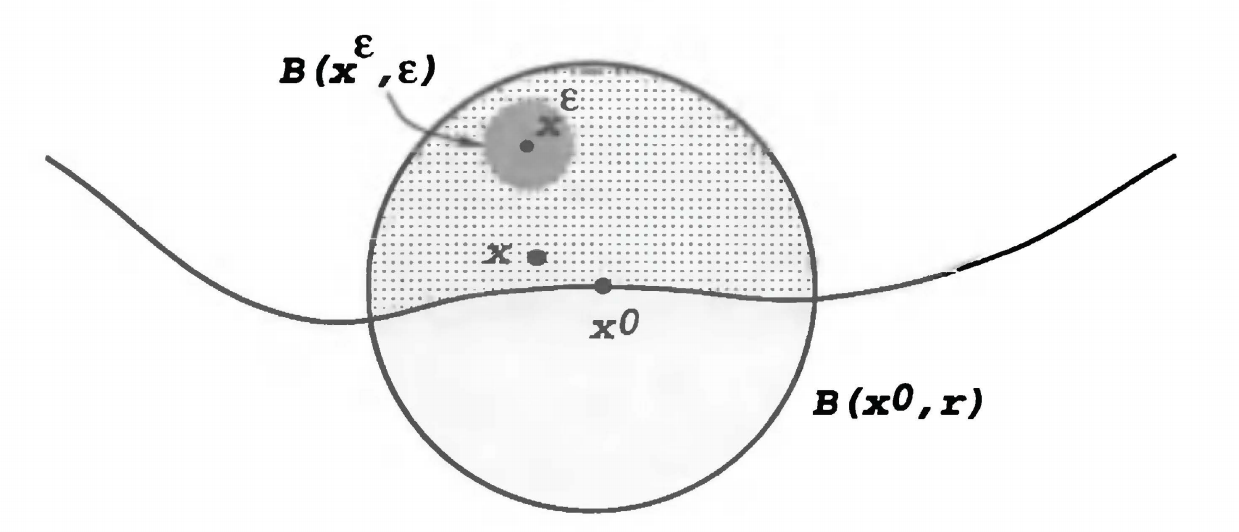
\includegraphics[scale=0.29]{Image/shift operator.png}
    \caption{The Shift Operator}
\end{figure}
\end{proof}
Now define $u_\varepsilon(x)=u(x^\varepsilon)$, where $x\in V$. This is a function translated from $u$ by a distance $\lambda\varepsilon$ in $e_n$ direction. Next we write $v^\varepsilon=\eta_\varepsilon*u_\varepsilon$. Trivially $v^\varepsilon\in C^\infty(\overline{V})$. We shall now claim $v^\varepsilon\to u$ in $W^{k,p}(V)$. It suffices to observe that 
$$
\left\| v^{\varepsilon}-u \right\| _{W^{k,p}\left( V \right)}^{p}=\sum_{\left| \alpha \right|\le k}{\left\| D^{\alpha}v^{\varepsilon}-D^{\alpha}u \right\| _{L^p\left( V \right)}^{p}}\le \sum_{\left| \alpha \right|\le k}{\left( \left\| D^{\alpha}v^{\varepsilon}-D^{\alpha}u_{\varepsilon} \right\| _{L^p\left( V \right)}+\left\| D^{\alpha}u_{\varepsilon}-D^{\alpha}u \right\| _{L^p\left( V \right)} \right) ^p}\rightarrow 0.
$$
Now since $\partial U$ is compact, we may select finite many points $x^0_i\in\partial U$ and radii $r_i$ such that 
$$
\partial U\subset \bigcup_{i=1}^N{B\left( x_{i}^{0},\frac{r_i}{2} \right)}.
$$
Define $V_i=U\cap B(x_i^0,r_i/2)$, then there exists $v_i\in C^\infty(\overline{V}_i)$ such that 
$$
\left\| v_i-u \right\| _{W^{k,p}\left( V_I \right)}\le \delta .
$$
Take an open set $V_0\subset\subset U$ such that $U\subset\bigcup_{i=0}^NV_i$, and select a function $v_0\in C^\infty(\overline{V}_0)$ such that 
$$
\left\| v_0-u \right\| _{W^{k,p}\left( V_I \right)}\le \delta .
$$
Now let $\{\zeta_i\}_{i=0}^\infty$ be a set of partitions of unity on $\overline{U}$, subordinate to the open sets 
$$
\left\{ V_0,B\left( x_{1}^{0},\frac{r_1}{2} \right) ,\cdots ,B\left( x_{N}^{0},\frac{r_N}{2} \right) \right\} .
$$
Define $v=\sum_{i=0}^N\zeta_iv_i$. Then by an analogous argument of Theorem \ref{Thm4.3.2} we finished our proof.
\subsection{Extensions}
Our goal next is to extend functions in the Sobolev space $W^{1,p}(U)$ to become functions in the Sobolev space $W^{1,p}(\mathbb{R}^n)$. We suppose $1\le p\le\infty$.
\begin{theorem}
Assume $U$ is bounded and $\partial U$ is $C^1$. Select a bounded open set $V$ such that $U\subset\subset V$. Then there exists a bounded linear operator $E:W^{1,p}(U)\to W^{1,p}(\mathbb{R}^n)$ such that for each $u\in W^{1,p}(U)$,\par
(i) $Eu=u$ a.e. in $U$,\par
(ii) $Eu$ has a support within $V$,\par
(iii) $\|Eu\|_{W^{1,p}(\mathbb{R}^n}\le C\|u\|_{W^{1,p}(U)}$, where the constant $C$ depends only on $p$, $U$ and $V$.
\end{theorem}
\begin{proof}
Fix $x^0\in\partial U$. Since we may consider $U$ as a submanifold of $\mathbb{R}^n$, we therefore suppose $\partial U$ is flat near $x^0$ and lying in the plane $\{x_n=0\}$, or otherwise we may choose $\Phi$ with inverse $\Psi$ such that "straightens out $\partial U$ near $x^0$".\par
\begin{figure}[htbp]
    \center
    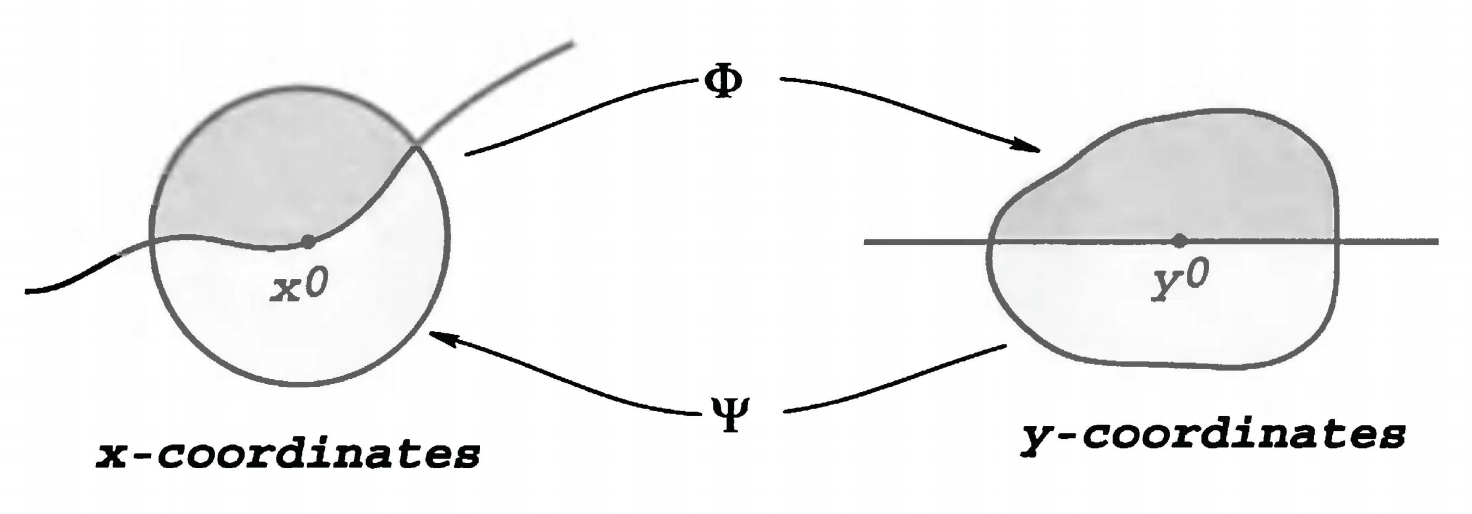
\includegraphics[scale=0.29]{Image/straightening out.png}
    \caption{Straightening Out the Boundary}
\end{figure}
Then we may assume there exists an open ball $B$, with center $x^0$ and radius $r$, such that 
$$
B^+=B\cap \left\{ x_n\ge 0 \right\} \subset \overline{U},\hspace{0.5cm}B^-=B\cap \left\{ x_n\le 0 \right\} \subset \mathbb{R} ^n\setminus U.
$$
We shall also suppose $u\in C^1(\overline{U})$ since by the approximation method we may use $C^\infty(\overline{U})$ functions to approximate $u$. We define 
$$
\overline{u}\left( x \right) =\left\{ \begin{aligned}
	u\left( x \right) &,\ x\in B^+\\
	-3u\left( x_1,\cdots ,x_{n-1},-x_n \right) +4u\left( x_1,\cdots ,x_{n-1},-\frac{x_n}{2} \right) &,\ x\in B^-\\
\end{aligned} \right. 
$$
we claim $\overline{u}\in C^1(\overline{B})$. Since the only possible discontinuous place is $\{x_n=0\}$, we compute each partial derivatives on $\{x_n=0\}$. Let $u^+=\overline{u}\mid_{B^+}$ and $u^-=\overline{u}\mid_{B^-}$. Note that 
$$
u_{x_n}^{-}\left( x \right) =3u_{x_n}\left( x_1,\cdots ,x_{n-1},-x_n \right) -2u_{x_n}\left( x_1,\cdots ,x_{n-1},-\frac{x_n}{2} \right) ,
$$
therefore $u_{x_n}^{-}\mid_{\{x_n=0\}}=u_{x_n}$. Similarly we have $u_{x_i}^{-}\mid_{\{x_n=0\}}=u_{x_i}$ and hence $D^\alpha u^-\mid_{\{x_n=0\}}=D^\alpha u^+\mid_{\{x_n=0\}}$ for each $|\alpha|\le 1$, and so $\overline{u}\in C^1(\overline{B})$.\par
Now we check the norm inequality. Note that 
$$
\begin{aligned}
\left\| \overline{u} \right\| _{W^{1,p}\left( B \right)}^{p}&=\sum_{\left| \alpha \right|\le 1}{\int_B{\left| D^{\alpha}\overline{u} \right|^p\mathrm{d}x}}
\\
&\le \sum_{\left| \alpha \right|\le 1}{\left( \int_{B^+}{\left| D^{\alpha}\overline{u} \right|^p\mathrm{d}x}+\int_{B^-}{\left| D^{\alpha}\overline{u} \right|^p\mathrm{d}x} \right)}
\\
&=\sum_{\left| \alpha \right|\le 1}{\left( \int_{B^+}{\left| D^{\alpha}u \right|^p\mathrm{d}x}+\int_{B^-}{\left| D^{\alpha}\overline{u} \right|^p\mathrm{d}x} \right)}
\\
&=\sum_{\left| \alpha \right|\le 1}{\left( \int_{B^+}{\left| D^{\alpha}u \right|^p\mathrm{d}x}+\int_{B^-}{\left| -3D^{\alpha}u\left( x_1\cdots ,-x_n \right) +4D^{\alpha}u\left( x_1\cdots ,-\frac{x_n}{2} \right) \right|^p\mathrm{d}x} \right)}
\\
&\le \sum_{\left| \alpha \right|\le 1}{\left( \int_{B^+}{\left| D^{\alpha}u \right|^p\mathrm{d}x}+3\int_{B^-}{\left| D^{\alpha}u\left( x_1, \cdots ,-x_n \right) \right|^p\mathrm{d}x}+4\int_{B^-}{\left| D^{\alpha}u\left( x_1, \cdots ,-\frac{x_n}{2} \right) \right|^p\mathrm{d}x} \right)}
\\
&=\sum_{\left| \alpha \right|\le 1}{\left( \int_{B^+}{\left| D^{\alpha}u \right|^p\mathrm{d}x}+3\int_{B^+}{\left| D^{\alpha}u \right|^p\mathrm{d}x}+4\int_{B^+\cap \left\{ x_n\le \frac{r}{2} \right\}}{2^{-p}\cdot \left| D^{\alpha}u \right|^p\mathrm{d}x} \right)}
\\
&\le \sum_{\left| \alpha \right|\le 1}{\left( \int_{B^+}{\left| D^{\alpha}u \right|^p\mathrm{d}x}+\max \left\{ 3,2^{2-p} \right\} \cdot \int_{B^+}{\left| D^{\alpha}u \right|^p\mathrm{d}x} \right)}
\\
&\le C\sum_{\left| \alpha \right|\le 1}{\int_B{\left| D^{\alpha}u \right|^p\mathrm{d}x}}=C\left\| u \right\| _{W^{1,p}\left( B^+ \right)},
\end{aligned}
$$
we therefore have 
$$
\left\| \overline{u} \right\| _{W^{1,p}\left( B \right)}\le C\left\| u \right\| _{W^{1,p}\left( B^+ \right)}.
$$
Now since $\partial U$ is $C^1$, we may use a partition of unity over $\partial U$ to extend our result to the global condition. To be explicit, suppose $\partial U\subset\bigcup_{i=1}^NW_i$. Choose $W_0$ such that $U\subset\bigcup_{i=0}^NW_i$ and suppose $\{\zeta_i\}_{i=0}^N$ be the associated partition of unity. Choose $x_i^0\in W_i$ and define $\overline{u}_i$ analogously. Now define $\overline{u}=\sum_{i=0}^N\zeta_i\overline{u}_i$, where $\overline{u}_0=u$. Therefore we have 
$$
\left\| \overline{u} \right\| _{W^{1,p}\left( \mathbb{R} ^n \right)}\le \left\| u \right\| _{W^{1,p}\left( U \right)}+\sum_{i=1}^N{\left\| \overline{u}_i \right\| _{W^{1,p}\left( B_i \right)}}\le \left\| u \right\| _{W^{1,p}\left( U \right)}+\sum_{i=1}^N{C_i\left\| u_i \right\| _{W^{1,p}\left( B_{i}^{+} \right)}}\le \max \left\{ 1,C_1,\cdots ,C_N \right\} \cdot \left\| u \right\| _{W^{1,p}\left( U \right)}.
$$
Therefore the norm inequality also holds. Furthermore we can arrange for the support of $\overline{u}$ to lie within $V\supset\supset U$.\par
We henceforth define $Eu=\overline{u}$ and now we show that $E$ is a bounded linear operator. Observe that 
$$
E\left( u+v \right) =\overline{u+v}=\sum_{i=0}^N{\zeta _i\cdot \left( \overline{u+v} \right) _i}=\sum_{i=0}^N{\zeta _i\left( \overline{u}_i+\overline{v}_i \right)}=\sum_{i=0}^N{\zeta _i\overline{u}_i}+\sum_{i=0}^N{\zeta _i\overline{v}_i}=Eu+Ev
$$
and 
$$
E\left( ku \right) =\overline{ku}=\sum_{i=0}^N{\zeta _i\left( \overline{ku} \right) _i}=\sum_{i=0}^N{k\cdot \zeta _i\overline{u}_i}=k\sum_{i=0}^N{\zeta _i\overline{u}_i}=kEu,
$$
we have $E$ a linear operator. By the norm inequality we have $E$ is bounded. Therefore the proof is finished.
\end{proof}
\begin{note}\em
We shall call $Eu$ an \textbf{extension} of $u$ to $\mathbb{R}^n$.\par
Assume now $\partial U$ is in $C^2$. Then the extension operator $E$ constructed above is also a bounded linear operator from $W^{2,p}(U)$ to $W^{2,p}(\mathbb{R}^n)$ since the reflection $\overline{u}$ lies in $W^{2,p}(B)$. We also have the norm inequality 
$$
\left\| Eu \right\| _{W^{2,p}\left( \mathbb{R} ^n \right)}^{p}\le C\left\| u \right\| _{W^{1,p}\left( U \right)}
$$
with $C$ only dependent on $n$, $p$, $U$ and $V$.\par
Note however, if $k>2$, then the construction before does not provide us an extension in $W^{k,p}(U)$. This requires a more complicated higher-order reflection principle and we shall first put it aside. 
\end{note}